\chapter{Do-Calculus}\label{chap-do-calc}


The do-calculus and associated ideas were
invented by
Judea Pearl and collaborators.
This chapter is 
based on Judea Pearl's
books. (See \ref{ch-nav-pearl}).


When
doing
do-calculus,
it is 
convenient
to separate
the nodes
of a bnet
into
2  types:
{\bf visible (observed)},
and {\bf non-visible (not observed,
hidden)},
depending
on
whether data
describing
the
state 
of that
node
is available 
(visible) or not (non-visible).
In this chapter, hidden nodes will 
be indicated 
in a bnet
diagram by
either: (1)
enclosing
their random variable
in a box (as
if it were inside a black box) or
(2) making
the arrows
coming
out of them
dashed.
Accordingly, 
the 
3 diagrams 
in
Fig.\ref{fig-hidden-dashes}
all mean the same thing.

A {\bf confounder node
for $\rvx$ and $\rvy$}
(such as node
$\rvc$
in Fig.\ref{fig-hidden-dashes})
is a hidden node 
with arrows
pointing
from it to
both
$\rvx$ and $\rvy$.
In other words, it's
an unobserved common
cause of $\rvx$ and $\rvy$.

In this book,
we will refer
to a path
all of whose nodes are
observed as an {\bf opath}.



\begin{figure}[h!]
$$\xymatrix{
&*+[F]{\rvc}\ar[dl]\ar[dr]
\\
\rvx\ar[rr]&&\rvy
}
\;\;\;
\xymatrix{
\rvx\ar@{-->}@{<-->}@/^2pc/[rr]
\ar[rr]&&\rvy
}
\;\;\;
\xymatrix{
&\rvc\ar@{-->}[dl]\ar@{-->}[dr]
\\
\rvx\ar[rr]&&\rvy
}$$
\caption{
These 3 diagrams
are equivalent.
They
mean that node $\rvc$
is hidden.
Node $\rvc$
is implicit
in the
middle diagram.}
\label{fig-hidden-dashes}
\end{figure}



Define
an
operator
$\rho_\rvx$
that acts on
a node
$\rvx$
of a bnet
to
delete
all
the 
arrows
entering
$\rvx$,
thus
coverting
$\rvx$
into
a new
node $\rho \rvx$
that
is a root node.
Define 
an analogous 
operator
$\lam\rvx$
that acts on
a node
$\rvx$
of a bnet
to
delete
all
the 
arrows
leaving
$\rvx$,
thus
converting
$\rvx$
into
a new
node $\lam \rvx$
that
is a leaf node.
$\rho_\rvx$
and
$\lam_\rvx$
are
depicted
in Fig.\ref{fig-do-rho-lam}.



\begin{figure}[h!]
\centering
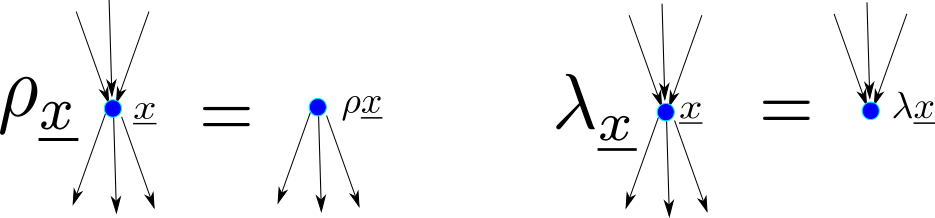
\includegraphics[width=4in]
{do/do-rho-lam.png}
\caption{
The operator $\rho_\rvx$
converts node $\rvx$
into a root node $\rho \rvx$.
The operator $\lam_\rvx$
converts node $\rvx$
into a leaf node $\lam\rvx$.
} 
\label{fig-do-rho-lam}
\end{figure}


If
you don't
know yet
what we mean by a
a multi-node
$\rva.$, see
Chapter \ref{ch-bnet-def}

Given a bnet
$G$,
we define
as follows
the operators
$\rho_{\rva.}$
and
$\lam_{\rva.}$
for a multi-node
$\rva.$.

\beq
\rho_{\rva.}G =
\left[\prod_j \rho_{\rva_j}\right]G
\;,\;\;\;\;
\lam_{\rva.}G =
\left[\prod_j \lam_{\rva_j}\right]G
\;.
\eeq

Consider a bnet 
whose totality of nodes
is labeled $\rvX.$.
Recall that 

\beq
P(X.)=
\prod_j P(X_j|(X_k)
_{k:\rvX_k\in pa(\rvX_j)})
\;.
\eeq

Define an
operator $\rho$
that acts as follows\footnote{As usual,
$\caln(!x)$ denotes 
a constant 
that is independent of $x$.}: Let
$X.-a.=(X_k)_{k:\rvX_k\notin \rva.}$.

\beqa
P(X.-a.|\rho\rva.=a.)
&=&
\caln(!(X.-a.))
\frac{P(X.)}
{
\prod_{j:\rvX_j\in \rva.}
P(X_j|(X_k)
_{k:\rvX_k\in pa(\rvX_j)})
}
\\
&=&
\caln(!(X.-a.))
\prod_{j:\rvX_j\notin \rva.}
P(X_j|(X_k)
_{k:\rvX_k\in pa(\rvX_j)})
\\
&\neq&
P(X.-a.|\rva.=a.)
\;.
\eeqa
Also,

\beq
P(X.-a.,\rho\rva.=a.')=
P(X.-a.|\rho\rva.=a.)
\delta(a'., a.)
\;.
\eeq
In words, we replace
the TPM for 
multinode
$\rva.$ by
a deterministic
prior
distribution.

For instance, for the bnet

\beq
\xymatrix{
\rvx\ar[r]&\rvy
}
\eeq
with 

\beq
P(x,y)=P(y|x)P(x)
\;,
\eeq
one has 

\beq
P(y|\rho\rvx=x)=P(y|x)
\eeq
and

\beq
P(x|\rho \rvy=y)=P(x)
\;.
\eeq
This means that $\rvx$ causes $\rvy$
and $\rvy$ does not cause $\rvx$.

For the bnet

\beq
\xymatrix{
\rvc\ar[d]\ar[rd]
\\
\rvx\ar[r]&\rvy
}
\eeq
with 

\beq
P(x,y, c)=P(y|x, c)P(x|c)P(c)
\;,
\eeq
one has 

\beq
P(y, c|\rho\rvx=x)=P(y|x, c)P(c)
\;.
\eeq
Hence,

\beq
P(y|\rho\rvx=x)=\sum_c P(y|x,c)P(c)
\;.
\eeq
This is called {\bf adjusting the parents
of $\rvx$}.

For
$\rvb.\subset \rvX.-\rva.$,
define

\beq
P(b.|\rho\rva. =a.)=
\sum_{X.-a.-b.}
P(X.-a.|\rho\rva.=a.)
\;,
\eeq
and for
$\rvs.\subset \rvX.-\rva.-\rvb.$,
define

\beq
P(b.|\rho \rva.=a., s.)=
\frac{P(b., s.|\rho\rva.=a.)}
{P(s.|\rho\rva.=a.)}
\;.
\eeq

$P(b.|\rho \rva.=a., s.)$
is usually denoted instead  by
$P(b.|do(\rva.=a.), s.)$.
I prefer to 
use $\rho$
instead of $do()$ to remind me that
it generates root nodes.
I'll still call $\rho$
a {\bf do operator}. 

In $P(y|\rho \rvx=x)$,
node $\rvx$ is turned 
into a root node. This guarantees
that there is
no confounding node
connecting $\rvx$ and
$\rvy$. Such 
confounding nodes 
are unwelcomed 
when calculating
causal effects
between 
the 2 variables $\rvx$ and $\rvy$
 because they 
 introduce 
non-causal
correlations between
the two.
This is also 
what happens
in a {\bf Randomized 
Clinical Trial (RCT)}.
In a RCT
 with treatment $\rvx$,
the value
of $\rvx$ for each patient
is determined by a coin toss,
effectively
turning $\rvx$ into a root node.
Hence, the do operator mimics a RCT.


$P(b.|\rho \rva.=a., s.)$
is said to be {\bf identifiable}
if it can be
expressed in terms of
probability distributions
that only
depend on observed 
variables and that
have no do operators
in them.
For example,
$P(y|\rho\rvx=x)$ is identifiable
for the bnet

\beq
\xymatrix{
\rvz\ar[d]\ar[dr]
\\
\rvx\ar[r]&\rvy
}
\eeq
but it is non-identifiable for the bnet

\beq
\xymatrix{
*+[F]{\rvz}\ar[d]\ar[dr]
\\
\rvx\ar[r]&\rvy
}
\eeq


For $\rvx, \rvy\in \bool$, the {\bf
causal effect difference} ,
or {\bf average causal effect (ACE)}
is defined as

\beq
ACE=
P(y=1|\rho \rvx=1)-
P(y=1|\rho \rvx=0)
\eeq
and the 
{\bf Risk Difference (RD)} as

\beq
RD=
P(y=1|\rvx=1)-
P(y=1|\rvx=0)
\;.
\eeq

\section*{Parent Adjustment}


Suppose 
that $\rvx., \rvy., \rvz.$
are disjoint multinodes
and their union equals
 the
totality of all nodes of
a bnet. 
Suppose we have data
available that allows us  to
estimate $P(x., y., z.)$.
Hence, all nodes of the bnet
are observable.
Furthermore,
suppose $\rvz.=pa(\rvx.)$.
In other words,
we are 
considering the bnet

\beq
\xymatrix{
\rvz.\ar[d]\ar[dr]
\\
\rvx.\ar[r]&\rvy.
}
\;.
\eeq

Then

\beq
P(y., z.|\rho \rvx.=x.)
=P(y.|x., z.)P(z.)
\eeq
so

\beq
P(y.|\rho \rvx.=x.)
=\sum_{z.}P(y.|x., z.)P(z.)
\;.
\eeq
This is called
{\bf adjusting the parents}
of $\rvx.$.


We say that 
we are {\bf adjusting 
or controlling a variable $\rva$}
if we condition 
a probability on $\rva$ and 
then we average 
that probability over $\rva$.
More generally, 
we can adjust a whole
multinode $\rva.$ together.

Later on,
we will introduce 
a generalization
of 
this parent adjustment
called the 
backdoor adjustment.
In a backdoor adjustment,
the adjusted multinode
is not necessarily
 the parents of $\rvx.$, 
and $P(x., y., z.)$
need not represent the
whole bnet.



\section*{3 Rules of do-calculus}
Throughout 
this section, suppose
$\rva., \rvb., \rvr., 
\rvs.$ are disjoint
multinodes in a bnet $G$.


Recall
from Chapter \ref{chap-dsep}
on d-separation,
that  $(\rvb.\perp \rva.|\rvr., \rvs.)$
means that 
we have established
from the d-separation
rules that 
that all 
paths in $G$
 from
$\rva.$ to
$\rvb.$
are blocked
if we condition
on $\rvr.\cup \rvs.$.
Recall also that:

\begin{itemize}
\item {\bf Rule 0:} Insertion or
 deletion of
 observations, without
do operators.
($\rva.=a. \leftrightarrow 1$ )


If 
 $(\rvb.\perp \rva.|\rvr., 
\rvs.)$ in $G$, then 
$P(b.|a., r., s.)=P(b.|r., s.)$
\end{itemize}

The 3 rules of do-calculus
can be presented in the same
format. 


\begin{color}{red}
\begin{itemize}
\item {\bf Rule 1:} 
Insertion or deletion of
 observations 
($\rva.=a. \leftrightarrow 1$ )

\ruleone

\item {\bf Rule 2:} Action or 
observation exchange 
($\rho \rva.=a. \leftrightarrow \rva.=a.$)

\ruletwo

\item {\bf Rule 3:} Insertion and
 deletion of actions
($\rho \rva.=a. \leftrightarrow 1$)

\rulethree


\end{itemize}
\end{color}

These rules have been
proven to be 
sufficient
for removing
all do operators
from an expression
for 
which it 
is possible to do so.

Next we discuss
two theorems that can be
proven using
do-calculus:
the backdoor and the
front-door
adjustment theorems.

The 
backdoor theorem 
adjusts one multinode
and the 
front-door theorem adjusts two.


\section*{Backdoor Adjustment}

See Chapter \ref{chap-bdoor}
for examples of the use of the 
backdoor adjustment theorem.
In this section,
we shall mainly be
concerned with
proving this
theorem
using do-calculus.



\bdoordef

{\bf Motivation for BD criterion}: 
Part 1 rules out
paths 
from $\rvx$
to $\rvy$
containing a fork node (confounder)
which, if not blocked by $\rvz.$, 
 would introduce a
non-causal correlation 
(confounder bias).
Part 2 rules out
a directed path
from $\rvx$ to $\rvy$
that has a mediator node
blocked by $\rvz.$
or a collider node
unblocked by $\rvz.$.



\begin{claim} Backdoor Adjustment Theorem

\bdoorclaim
\end{claim}
\proof

For simplicity,
let us omit
the dots from the
multinodes.
If
$z$
satisfies the
backdoor
criterion
relative
to
$(\rvx, \rvy)$,
then
$\rvx, \rvy, \rvz$
must 
have the following 
structure.


\beq
\xymatrix{
{\rvz}\ar[d]\ar[rd]
\\
\rvx\ar[r]&\rvy
}
\eeq
\beq
\begin{array}{lllll}
&&\color{red}
P(y|\rho\rvx=x)=
\\
&=&
\color{red}
\sum_m 
P(y|\rho\rvx=x, z)
P(z|\rho\rvx=x) 
\\
&&\text{by Probability Axioms}
\\
&=&\color{red}
\sum_ 
P(y|x, z)
P(z|\rho\rvx=x)
\\
&&P(y|\rho \rvx=x, z)\rarrow
P(y|x, z)
\\
&& \text{ by Rule 2: \ruletwo}
\\
&&
\rvy\perp \rvx|\rvz
\text{ in }\lam_\rvx G
\;\;\;\;
\xymatrix{
{\rvz}\ar[d]\ar[rd]
\\
\rvx&\rvy
}
\\
&=&\color{red}
\sum_z 
P(y|x, z)
P(z)
\\
&&P(z|\rho \rvx=x)\rarrow
P(z)
\\
&& \text{ by Rule 3: \rulethree}
\\
&&
\rvz\perp \rvx
\text{ in }\rho_\rvx G
\;\;\;\;
\xymatrix{
{\rvz}\ar[rd]
\\
\rvx\ar[r]&\rvy
}
\end{array}
\eeq
\qed

Note that the backdoor adjustment  formula
can be written as
 
\beqa
P(y.|\rho \rvx. =x.)
&=&
\sum_{z.}P(y.|x., z.)P(z.)
\\
&=&
\sum_{z.}\frac{P(y.,x., z.)}
{P(x.|z.)}
\eeqa
This assumes $P(x.|z.)\neq 0$
for all $x., z.$. This assumption
is referred to
as {\bf positivity},
and is violated
if $P(x.|z.)=\delta(x., x.(z.))$.
$P(x.|z.)$ is called the 
{\bf propensity score}
of $x.$ given $z.$.
This
equation does 
{\bf inverse probability weighting}.
One
can approximate $P(x.|z.)$ 
in this equation
to get
an approximation
to  $P(y|\rho\rvx=x)$.


\section*{Front Door Adjustment}
See Chapter \ref{chap-fdoor}
for examples of the use of the 
front-door adjustment theorem.
In this section,
we shall mainly be
concerned with
proving this
theorem
using do-calculus.

\fdoordef

\begin{claim} Front-Door Adjustment
Theorem

\fdoorclaim

\end{claim}
\proof

For simplicity,
let us omit
the dots from the
multinodes.
If
$\rvm$
satisfies the
front-door
criterion
relative
to
$(\rvx, \rvy)$,
then
$\rvx, \rvm, \rvy$
must 
have the following 
structure,
where
node $\rvc$
is hidden. 



\beq
\xymatrix{
&*+[F]{\rvc}\ar[ld]\ar[rd]
\\
\rvx\ar[r]&\rvm\ar[r]&\rvy
}
\eeq

Continues in next page.
\newpage
\beq
\begin{array}{lllll}
&&\color{red}
P(y|\rho\rvx=x)=
\\
&=&
\color{red}
\sum_m 
P(y|\rho\rvx=x, m)
P(m|\rho\rvx=x) 
\\
&&\text{by Probability Axioms}
\\
&=&\color{red}
\sum_m 
P(y|\rho\rvx=x, \rho\rvm=m)
P(m|\rho\rvx=x)
\\
&&P(y|\rho\rvx=x, m)\rarrow
P(y|\rho\rvx=x, \rho m=m)
\\
&& \text{ by Rule 2: \ruletwo}
\\
&&
\rvy\perp \rvm|\rvx
\text{ in }\lam_\rvm\rho_\rvx G
\xymatrix{
&*+[F]{\rvc}\ar[rd]
\\
\rvx\ar[r]&\rvm&\rvy
}
\\
&=&\color{red}
\sum_m 
P(y|\rho\rvx=x, \rho\rvm=m)
P(m| x)
\\
&&
P(m|\rho\rvx=x)\rarrow P(m|x)
\\
&&\text{by Rule 2: \ruletwo}
\\
&&
\rvm\perp\rvx
\text{ in }
\lam_\rvx G
\xymatrix{
&*+[F]{\rvc}\ar[ld]\ar[rd]
\\
\rvx&\rvm\ar[r]&\rvy
}
\\
&=&\color{red}
\sum_m 
P(y|\rho\rvm=m)
P(m|x)
\\
&&
P(y|\rho\rvx=x, \rho\rvm=m)
\rarrow
P(y|\rho\rvm=m)
\\
&&\text{by Rule 3: \rulethree}
\\
&&
\rvy\perp\rvx|\rvm
\text{ in }
\rho_\rvx\rho_\rvm G
\xymatrix{
&*+[F]{\rvc}\ar[rd]
\\
\rvx&\rvm\ar[r]&\rvy
}
\\
&=&\color{red}
\sum_{x'}
\sum_m 
P(y|\rho\rvm=m, x')
P(x'|\rho\rvm=m)
P(m|x)
\\
&&\text{by Probability Axioms}
\\
&=&\color{red}
\sum_{x'}
\sum_m 
P(y|m, x')
P(x'|\rho\rvm=m)
P(m|x)
\\
&&
P(y|\rho\rvm=m, x')
\rarrow
P(y|m, x')
\\
&& \text{by Rule 2: \ruletwo}
\\
&&
\rvy\perp\rvm|\rvx
\text{ in }
\lam_\rvm G
\xymatrix{
&*+[F]{\rvc}\ar[rd]\ar[ld]
\\
\rvx\ar[r]& \rvm&\rvy
}
\\
&=&\color{red}
\sum_{x'}
\sum_m 
P(y|m, x')
P(x')
P(m|x)
\\
&&
P(x'|\rho\rvm=m)
\rarrow
P(x')
\\
&&\text{by Rule 3: \rulethree}
\\
&&
\rvx\perp\rvm
\text{ in }
\rho_\rvm G
\xymatrix{
&*+[F]{\rvc}\ar[rd]\ar[ld]
\\
\rvx&\rvm\ar[r]&\rvy
}
\end{array}
\eeq
\qed


